\section{Lecture 13}

\subsection{Inverse Mapping Theorem - Continued}

Recall that per the setting of the Inverse Mapping Theorem:
\begin{itemize}
    \item Let $f \in Hol(\Omega)$ and $z_0 \in \Omega$, $f(z_0) = w_0$ and $f'(z_0) \neq 0$
    \item $G$ is a bounded domain such that $cl(G) \subset \Omega$ (in textbook we choose $D_{z_0, p}$) and $\partial G \in PC^1$
    \item $|f(\xi) - w_0| \geq \delta$ for all $\xi \in \partial G$
    \item $f(z) \neq w_0 \forall z \in G$ (possible because all zeroes of non-constant analytic functions are isolated)
\end{itemize}

\begin{theorem}[Inverse Function Theorem]
Given the setup above, then for all $w$ such that $|w - w_0| < \delta$, there exists a unique $z$ in $G$ such that $f(z) = w$ and
\[f^{-1}(w) = z = \frac{1}{2\pi i} \int_{\partial G} \frac{\xi f'(\xi)}{f(\xi) - w} d\xi\]
\end{theorem}

\begin{proof}
\textbf{Existence and uniquenss are given by Rouche's Theorem.} Indeed, by the Argument Principle, we note that
\[\# \text{ of zeroes of $f(z) - w$ in $G$ } = \frac{1}{2\pi i} \int_{\partial G} \frac{f'(\xi)}{f(\xi) - w} d\xi\]
We note that we can rewrite
\[f(z) - w = [f(z) - w_0] + [w_0 - w]\]
\[|f(z) - w_0| \geq \delta, |w_0 - w| < \delta, \text{ on $\partial G$}\]
So Rouche's Theorem tells us that $f(z) - w$ and $f(z) - w_0$ has the same number of zeroes. But we note that we chose $f(z) - w_0$ to only have one zero, and it's a zero of order $1$ by condition given, so in other words $f(z) - w$ has exactly $1$ solution, hence uniqueness and existence are both proven.\\\\
\textbf{For the formula given, } we first note that the formula
\[\frac{\xi f'(\xi)}{f(\xi) - w}\]
has a unique singularity at $\xi = f^{-1}(w)$, which is a pole of order $1$ by construction. We can calculate its residue as
\begin{align*}
    Res(\frac{\xi f'(\xi)}{f(\xi) - w}, \xi = z) &= \lim_{\xi \to z} \frac{\xi f'(\xi)}{f(\xi) - w} \cdot (\xi - z)\\
    &= z f'(z) \lim_{\xi \to z} \frac{\xi - z}{f(\xi) - w}\\
    &= z f'(z) \lim_{\xi \to z} \frac{\xi - z}{f(\xi) - f(z)} \tag*{$w$ is defined to be $w = f(z)$}\\
    &= z f'(z) \frac{1}{f'(z)}\\
    &= z
\end{align*}
Then apply Cauchy's Residue Theorem gives us
\begin{align*}
    \frac{1}{2\pi i} \int_{\partial G} \frac{\xi f'(\xi)}{f(\xi) - w} d\xi &= \frac{2\pi i}{2\pi i} Res(\frac{\xi f'(\xi)}{f(\xi) - w}, \xi = z)\\
    &= Res(\frac{\xi f'(\xi)}{f(\xi) - w}, \xi = z)\\
    &= z\\
    &= f^{-1}(w)
\end{align*}
\end{proof}

Note that the local solvability of $f$ is just a standard result that can follow from Real Analysis too. However, the formula is more significant.

\subsection{Winding Numbers}

Let $\gamma: [a, b] \to \Cbb$ be a continuous function such that $\gamma(a) = \gamma(b)$ (This is a $C^0$-closed-path). We will denote $\Gamma$ as the image of $\gamma$ in $\Cbb$.\\

Without loss of generality, we can view $\gamma$ as a function:
\[\gamma: \Tbb \to \Cbb\]
, where $\Tbb \coloneqq \frac{\Rbb}{\Zbb}$ is the $1$-dimensional torus given by an equivalence relation on $\Rbb$, where we say $a \sim b$ if $a - b \in \Zbb$.

\begin{definition}
Let $\gamma$ be as before and let $z \in \Cbb \setminus \Gamma$, then we define the \textbf{winding number} as
\[w(\gamma, z) \coloneqq \frac{1}{2\pi i} \int_{\Gamma} \frac{1}{\xi - z} d\xi\]
\end{definition}

\begin{proposition}
$w(\gamma, z)$ is an integer valued function.
\end{proposition}

\begin{proof}
The proof is similar to the idea behind the Argument Principle, but we do not assume $\gamma$ is $C^1$. We first use the Lebesgue Number Lemma to split $\Gamma$ into small enough intervals such that $\frac{1}{\xi - z}$ locally has anti-derivatives on each interval (up to the choice of some branch):
\[log(\xi - z) + 2\pi i k, k \in \Zbb\]
As we move from one interval to another, we want to continue the branch we are previously on. We don't know what the branch is exactly, but this would form a telescoping series of primitivies, and the entire integral will evaluate to
\begin{align*}
    \frac{1}{2\pi i} \int_{\Gamma} \frac{1}{\xi - z} d\xi &= \frac{1}{2\pi i} [log(\xi - z) + 2\pi i k_1 - log(\xi - z) - 2\pi i k_2]\\
    &= \frac{2\pi i}{2\pi i}(k_1 - k_2)\\
    &= k_1 - k_2 \in \Zbb
\end{align*}
\end{proof}

\begin{proposition}
$w(\gamma, z)$ measures the number of times (sign given by whether it's counter-clockwise or clockwise) $\gamma$ wraps around $z$.
\end{proposition}

\begin{proof}[Proof Idea]
We note that $\gamma$ is homotopy equivalent to a circle, so the value of the integral doesn't change if we switch $\gamma$ to a circle of some positive radius around $z$. The branch choice given in the previous proposition actually follows in a circle (when viewed as a Riemann Surface), so the loop on the circle does measure the numbers of times it wraps around $z$. This is an invariant around homotopy equivalence.
\end{proof}

\begin{definition}
We say that $\gamma$ is a \textbf{generalized path} if $\gamma: \Tbb_1 \sqcup \Tbb_2 ... \sqcup \Tbb_n \to \Cbb$ and $\gamma$ restricted to each $\Tbb_k$ is a $C^0$-closed-path. In other words, $\gamma$ is intuitively the disjoint union of finitely many closed paths.
\end{definition}

\begin{remark}
Let $\gamma$ be a generalized path, and consider the function $z \mapsto W(\gamma, z)$. This is a well-defined function on $\Cbb \setminus Im(\gamma)$ and is moreover analytic on the same domain (this follows from Morera's Theorem). Thus, analyticity implies continuity, and for $W(\gamma, z)$ to be a continuous integer value, this means that $W(\gamma, z)$ is constant on each connected component of $\Cbb \setminus Im(\gamma)$. We sometimes call this the \textbf{index} of $\gamma$ at $z$.
\end{remark}

\subsection{Generalized Residue Theorem}

\begin{theorem}[Generalized Residue Theorem]
Let $\gamma$ be a generalized path in $\Omega$, and say $f \in Hol(\Omega \setminus \{z_1, ..., z_n\})$, and suppose for all $k$, $z_k \not \in Im(\gamma)$. Then
\[\int_{\gamma} f(z) dz = 2 \pi i \sum_{k = 1}^n w(\gamma, z_k) \cdot Res(f, z_k)\]
\end{theorem}

Before, we prove this theorem, we will introduce another theorem.

\begin{theorem}\label{thm::zero_path_thm}
Let $\gamma$ be a generalized path in $\Omega$, such that
\[W(\gamma, z) = 0, \text{ for all } z \not \in \Omega\]
(Note that this is true for any simply connected domain $\Omega$. If $\Omega$ has holes, then this is say that $\gamma$ avoids these holes). Then we have that
\[\int_\gamma f(z) dz = 0, \text{ for all $f \in Hol(\Omega)$}\]
\end{theorem}

\begin{proof}
Textbook (to be added)
\end{proof}

It turns out that Theorem~\ref{thm::zero_path_thm} actually implied the Generalized Residue Theorem.

\begin{proof}[Proof of the Generalized Residue Theorem]
Consider contours $\gamma_1, ..., \gamma_n$ be circles of small enough radius, each wrapping around $z_1, ..., z_n$ counterclock direction:
\[\fbox{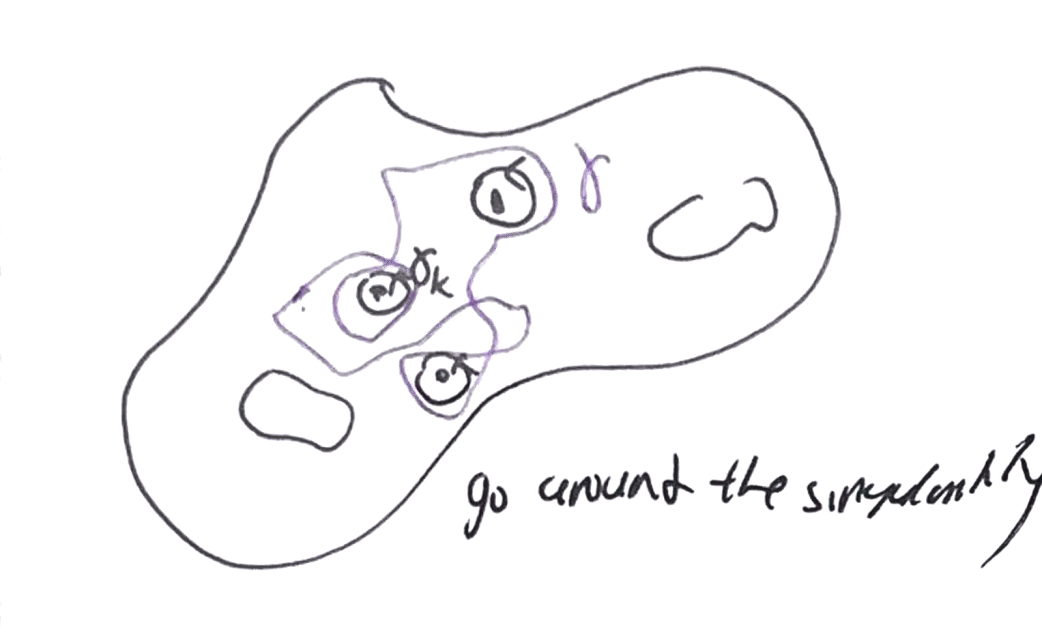
\includegraphics[width=.5\textwidth]{Figures/gen_path.png}}\]
Then consider the path $\hat{\gamma}$ given by
\[\hat{\gamma} \coloneqq \gamma - \bigcup_{k = 1}^n W(\gamma, z_k) \gamma_k\]
Then we note that for all $z \not in \Omega$, $W(\hat{\gamma}, z) = 0$ because the index of $\hat{gamma}$ at these points is reduced to $0$.\\\\
So Theorem~\ref{thm::zero_path_thm} tells us that
\begin{align*}
    0 &= \int_{\hat{\gamma}} f(z) dz\\
    &= \int_{\gamma} f(z) dz - \sum_{k = 1}^n \int_{\gamma_k} W(\gamma, z_k) f(z) dz\\
    &= \int_{\gamma} f(z) dz - [2 \pi i \sum_{k = 1}^n w(\gamma, z_k) \cdot Res(f, z_k)]
\end{align*}
\end{proof}